\usepackage{lipsum}
\usepackage[automake,toc]{glossaries}
\usepackage{caption}
\usepackage{listings}
\usepackage{xcolor}
\usepackage{filecontents}
\makeglossaries
% Term definitions 

\begin{document}

% =======================================================================================
%\cleardoublepage % Forces the first chapter to start on an odd page so it's on the right

% =======================================================================================
%                                   PREAMBLE
% =======================================================================================
\coverpage{\TITLE}{\SUBTITLE}{\AUTHOR}{\DATE}{\SUBJECT}
%----------------------------------------------------------------------------------------
\newpage
\tableofcontents

% =======================================================================================
%                                   PART I
% =======================================================================================
\part{Introduction to Cardano Smart Contracts}
%----------------------------------------------------------------------------------------
\newpage
\chapter{Overview of Cardano Blockchain} \label{ch:overview}
\subsection{History} \label{sec:overview}

Charles Hoskinson, along with Jeremy Wood, co-founded Cardano, both were part of Ethereum before. In 2015, they established Input Output Hong Kong to create and develop more sustainable blockchain solutions. Utilizing a peer-reviewed approach to blockchain development and introducing a novel consensus mechanism called \textbf{Ouroboros}, Cardano was prepared for its Mainnet launch in 2017.

\subsection{Ouroboros}

Ouroboros relies on a \textbf{proof of stake} consensus. Rather than requiring nodes to engage in computationally intensive work as in PoW chains, nodes are randomly selected based on the amount of ADA they hold at stake. This approach serves two purposes: it is more energy-efficient and incentivizes nodes to act responsibly as their stake is at risk in case of misbehavior.

\subsection{Cardano Architecture}

The blockchain model comprises several components. Users interact with the current ledger state by creating transactions, which are then submitted to the mempool until they are included in a block. Blocks are mined by stake pools, which are rewarded for their efforts and share these rewards with their delegators. Increased decentralization is achieved with more stake pool operators.
\subsection{Improvements from Other Blockchains}

Cardano offers several advantages over other chains:

\begin{itemize}
  \item \textbf{\textit{\gls{Determinism}}}: This feature enables transaction chaining.
  \item \textbf{Predictable Fees}: There is no risk of pending transactions due to fee increases.
  \item \textbf{Sustainability}: Unlike PoW, which is power-intensive, Cardano's approach is more sustainable.
  \item \textbf{Native Tokens}: Tokens are stored on the ledger, allowing smart contracts to interact with them. Users have control over tokens in their wallets, which cannot be frozen by external parties.
\end{itemize}

Scaling is currently the most significant challenge for the ecosystem. The ability to handle high volumes of users without being limited by block or transaction size is crucial for increasing adoption.

\subsection{\textit{Determinism} and predictable fees to make a better user experience}
Why \textbf{\textit{Determinism}} is important in smart contract programming?
Cardano inherits determinism from Bitcoin, once all the fields of a transaction are decided you will always get the same transaction Hash.
But more importantly, if you can get the hash of a transaction before actually submitting, you can even create a following transaction, relying on the first one.
This is usually called transaction chaining, I can create a chain of transactions that are not submitted, and this can allow me to speed up the user flow.
Ok, let's try to simplify even more this concept.
\begin{itemize}
  \item Alice, Bob and Raul are in a Bar, each has 100 ADA
  \item Alice sends to Raul 50 ADA but the blockchain right now is super clogged
  \item However Raul is already able to build a transaction to send 120 ADA to Bob because even if the blockchain is clogged, the hash of the transaction is already decided and won't change at all
  \item Now even Bob can send 220 ADA to someone else, even before the transactions are confirmed, due to Cardano determinism he can use transactions that are not confirmed yet
\end{itemize}

Everything seems amazing, perfect. Where is the issue?
What happens if for some reason Alice had her transaction with a deadline of 1 hour?
In that case, Alice's transaction could never become valid, therefore every other transaction depending on that will never make it.
This means that everything goes to the beginning, Alice, Bob and Raul have 100 ADA each. This is a problem if each of them paid for goods in the real world and now they get their money back.

Why do predictable fees matter and what's their role in \textit{determinism}?

On Bitcoin when you set inputs (what you spend), outputs (who gets the money) and fees you can get the transaction hash.
This happens also on Cardano, however on Bitcoin, there is a fee market, therefore the fees you set may not be enough to cover the cost of having the transaction in the next blocks.
So on Bitcoin fees may need to change, there is an RBF feature that allows you to speed up a transaction increasing the fee cost.
But this also leads to a change in the transaction hash, therefore we can't always build a chain of transactions on Bitcoin because one transaction could change, making all the following invalid.

On Cardano there is no fee market, in this way, once you pay enough to cover the processing costs, that transaction will be in the following blocks. Fees are not dynamic and can't change.

Even if it sounds cool, this leads to a problem, if there is no way of speeding up my transaction or making it possible to get priority over others, how can a protocol that needs instant settlement work?
This is an open question that lately has been discussed as a tier fee market on Cardano.

\newpage


\section{Importance and Applications of Smart Contracts}

Smart contracts are a concept born alongside Ethereum, enabling the execution of code and interactions without a third party. Once initiated, the terms of the contract are set by the parties involved, and no one can stop or interfere thereafter.

However, history teaches us that some protocols have included backdoors within their smart contracts, leading to fund theft or enabling bad actors to access users' funds.

Let's start with the basics.

\subsection{What is a Smart Contract?}

A smart contract is a decentralized software accessible to users on the blockchain, typically through a website interface. Users interacting with the contract can perform operations (financial, trading, storage) without requiring permission from a third party.

The essential components of a smart contract are:

\begin{itemize}
  \item \textbf{Parties}: Who can interact with the contract? Is it open to everyone, specific users, or owners of particular assets?
  \item \textbf{Actions}: What operations can users perform with the contract? These could include depositing funds, creating NFTs, storing data, reading data, withdrawing funds, and more.
  \item \textbf{Rules}: Define the actions each party can take under specific conditions.
  \item \textbf{Data Fields}: What data is involved in interactions with the contract, and how can each step of the interaction be tracked?
\end{itemize}
\subsection{Applications}

In a typical decentralized exchange (DEX) application, the parties are liquidity providers and traders. Liquidity providers can deposit and withdraw liquidity, while traders can only perform swaps. Rules dictate that liquidity providers must hold LP tokens in their wallets, while traders must have sufficient funds to cover transactions. Data fields stored in the contract typically include LP tokens, fees for liquidity providers, and token data.

In a marketplace scenario, the parties are sellers and buyers. Sellers can sell assets, while buyers can buy them. Rules stipulate that sellers must possess the assets they intend to sell, and buyers must have sufficient funds to purchase assets and pay sellers. Data stored includes the seller's address, payment amounts, royalties (if applicable), and platform fees.

On Cardano, specific actions might include \textbf{\textit{Cancel Listing}} and \textbf{\textit{Buy}}. \textbf{\textit{Selling/List}} is more of a smart contract interaction than an action.

\begin{remark}
  A smart contract action involves a transaction where the smart contract is invoked in the inputs. If the smart contract is present only in the outputs, it's considered a smart contract interaction.
\end{remark}

There can be many more smart contract applications, imagination is the limit, and some applications may work better on Cardano due to UTXO architecture or on EVM chains due to the account model.
Let's consider the case of a dex, it can be either \textbf{\textit{\gls{orderbook}}} or \textbf{\textit{\gls{AMM}}}. The orderbook works perfectly in a UTXO blockchain because every order can be a single UTXO.
While on EVM chains orderbook dexes struggle because they are limited by the memory of the smart contract.
On the opposite side, building an AMM on Cardano requires a lot of emulation, since the pool is a single UTXO, more parties can't spend it at the same time, that's why we found as solutions the batchers.
Batchers match the orders with the single UTXO liquidity pool.
This concept is not efficient however AMM are more user-friendly usually and that's why currently Cardano is the one leading in liquidity volumes.

\subsection{Smart Contract audits}

Once a smart contract is developed and ready to launch an audit should be done, this is to ensure that the code is safe and no issues may arise once people start interacting with it.
Audits play a critical role in the deployment of smart contracts, serving as a crucial safeguard against potential vulnerabilities and ensuring the integrity of the code.
Smart contracts, being immutable, leave little room for error once deployed, making thorough scrutiny prior to launch imperative.
Audits help identify security flaws, logic errors, and vulnerabilities that may compromise the contract's functionality or jeopardize users' funds.
By subjecting the code to rigorous review by experienced professionals, audits instill confidence among users and investors, fostering trust in the decentralized ecosystem. Moreover, audits contribute to the overall maturation of the blockchain space, driving standards for secure coding practices and enhancing the reliability of smart contract applications.
Ultimately, investing in audits upfront mitigates the risk of costly exploits or breaches down the line, safeguarding both the project's reputation and the interests of its stakeholders.

But audits have a cost and sometimes early projects may not afford that much.

Opensource can be a way in order to launch a project asking for external reviews coming from the community, usually bug bounty programs are run in order to incentivize users to collaborate in the task of finding risks in the smart contract code.

\subsection{Smart Contract risks}

On Cardano there are some risks regarding smart contracts that we'll study better in the following chapters, but here are a few of them as a preview:

\begin{itemize}
  \item Double satisfaction attack: User may spend two inputs that require similar conditions
  \item Dust attack: Users may add spam tokens in a smart contract making it impossible to retrieve funds from it
  \item Spam Contract: A second smart contract can run together with the attacked one, making it possible to unlock funds from the first
  \item Datum attack: A datum of the contract may be corrupted making unspendable the funds inside the contract
  \item backdoor: All the funds of the contract may be retrieved by someone who coded a backdoor
\end{itemize}

\subsection{The cost of deploying a contract}

Deploying a contract onto the blockchain carries no direct cost, allowing widespread accessibility. However, it's essential to consider additional expenses, especially if utilizing reference scripts like ADA, which may necessitate funds for storage on the blockchain. Moreover, while users typically prefer interacting with contracts via frontends, developing and maintaining such interfaces entail both frontend and backend costs. It's imperative to conduct thorough economic assessments before project launch, ensuring expenses don't surpass revenues. Abruptly discontinuing services without prior notice could result in users losing their funds, highlighting the importance of transparent communication in managing smart contract projects.
\section{Advantages of Cardano for Smart Contract Development}

Two years ago, if you asked me about the advantages of writing smart contracts on Cardano, I would have struggled to answer. However, now I can easily list several:

\begin{itemize}
  \item \textbf{\gls{Composability}}: The ability to create a transaction involving multiple contracts and perform actions with each of them.
  \item \textbf{User-Friendly}: No longer requiring Haskell, languages like Aiken, Opshin, and more offer a user-friendly experience.
  \item \textbf{\gls{Liquid Staking}}: Thanks to Cardano staking, smart contracts can delegate ADA or keep funds staked with liquidity providers.
  \item \textbf{UTxO Skills}: While much of the focus has been on Ethereum Virtual Machine (EVM) smart contracts, the UTXO model is ideal for solutions like ZK rollups, as it's easier to implement compared to the account model.
\end{itemize}

If you're still interested in becoming a Cardano smart contract wizard after this introduction, we can continue in the next chapter, where we'll install the components needed to \textbf{build on Cardano}.

% =======================================================================================
%                                   PART II
% =======================================================================================
\part{Setting Up the Development Environment}
%----------------------------------------------------------------------------------------
\newpage
\chapter{Installing and Configuring Cardano Development Tools} \label{ch:setup}
\section{Installing and Configuring Cardano Development Tools}\label{sec:setup}
The purpose of this book is to gather all the information for developing Cardano that currently is scattered around.
What are we going to use for our project?


\begin{itemize}
    \item \textbf{A hot Wallet}: We are going to use a wallet to test our contracts, this wallet will be used to receive tADA. We'll never store our main ADA holdings in this wallet: Wallets recommended for testnet are Nami on desktop and  Vespr for mobile.
    \item \textbf{A indexer account}: Indexers are the ones that will provide us the APIs in order to interact with the chain, we won't need to run a node for testing, let's use services and projects already there like \textbf{Maestro}, let's set up an account and get the API key.
    \item \textbf{Lucid library}: Lucid is not maintained anymore as a function and has been replaced by COMING SOON, however for testing and understanding the flow of Cardano transactions it can be really useful.
    \item \textbf{tADA}: How are we going to test without having testnet ADA? let's not mess up real ADA
    \item  \textbf{IDE}: Personally I use Visual Studio Code as IDE, but any other editor is ok since we are going to 
    \item \textbf{Cardano Node:} This is NOT mandatory at all, as homework, we could try to set up a Cardano node and interact with the chain using cardano-cli (command line), however, this is something we can do in our free time, there are other hobbies out there better than this, swimming, dancing or reading a book.
\end{itemize}

\section{Hot wallets on Cardano}
When it comes to the wallet choice on Cardano the question we should ask ourselves is: Desktop or Mobile?

\begin{table}[h!]
    \caption{Current Cardano wallets available, updated in Q2 24}
    \begin{tabular}{llll}
    Wallets & Desktop & Mobile & Website                    \\
    Nami    & X       &        & https://www.namiwallet.io/ \\
    Eternl  & X       & X      & https://eternl.io/         \\
    Begin   &         & X      & https://begin.is/          \\
    Vespr   &         & X      & https://vespr.xyz/         \\
    Lace    & X       &        & https://www.lace.io/       \\
    NuFi    & X       &        & https://nu.fi/             \\
    Yoroi   & X       & X      & https://yoroi-wallet.com/  \\
    Flint   & X       & X      & https://flint-wallet.com/  \\
    Gero    & X       &        & https://www.gerowallet.io/ \\
    Typhon  & X       &        & https://typhonwallet.io/   \\
    \end{tabular}
\end{table}

Test the wallet you like most and pick the one that gives you more user-friendly vibes for your use, a developer may require a very detailed wallet, however, a basic user may need just some very simple buttons without details.

\section{Setting Up and Connecting to Cardano Testnet}
So let's install a wallet and config for testnet 

In this example, we'll install the Nami wallet that we can find \href{https://www.namiwallet.io/}{here}

Once we install the wallet we'll get 24 seed phrase words

\begin{remark}
Never share the seedphrase or store it on a cloud, use paper or different ways to store it, software can keep track of your seedphrase and you could lose the funds.
\end{remark}

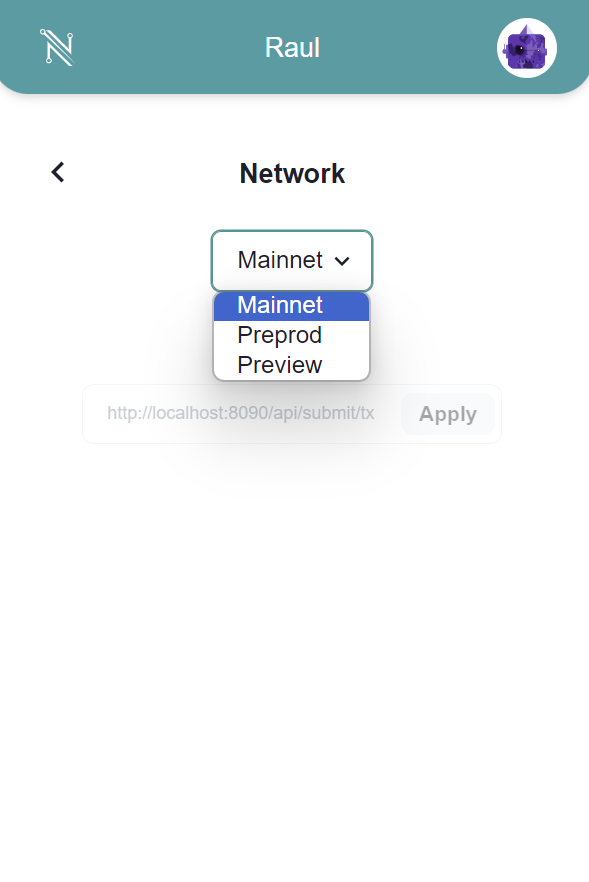
\includegraphics{wallet_preview}

Let's set Nami to \textbf{testnet preview} and we'll finally get our wallet in testnet 

\subsection{Preview and Preprod testnets}

\begin{itemize}
    \item \textbf{Mainnet}: This is the live network where real transactions occur using actual ADA. It's the primary arena where users engage with Cardano wallets, exchanges, and decentralized applications (dApps).
    \item \textbf{Preprod}: Acting as a staging ground for major upgrades and releases, Preprod is a testing environment where developers validate changes before deploying them to the mainnet. Utilizing test ADA acquired from the faucet, developers simulate real-world scenarios, ensuring everything functions as intended before the changes go live. Preprod typically mirrors mainnet's structure, forking nearly simultaneously to ensure alignment.
    \item \textbf{Preview}: Serving as a testing environment to showcase upcoming features and functionality, Preview allows developers and users to explore and provide feedback on new developments before they reach the wider community. Like Preprod, test ADA from the faucet facilitates testing. Notably, Preview precedes mainnet hard forks by a minimum of four weeks, offering ample time for thorough evaluation and refinement based on community input.
\end{itemize}

\subsection{Get tADA}

In order to receive tADA we can use the official faucet from Cardano at the following \href{https://docs.cardano.org/cardano-testnets/tools/faucet/}{link}

The process doesn't involve any payment and at the end of your testing, ideally, you should return tADA back so other devs can work with it.

\subsection{CIP30}

To connect our wallet with any webpage we'll use \gls{CIP}30 reference, we can find the list of methods to connect and invoke the functions of the wallets at this \href{https://www.cardano-caniuse.io/}{page}

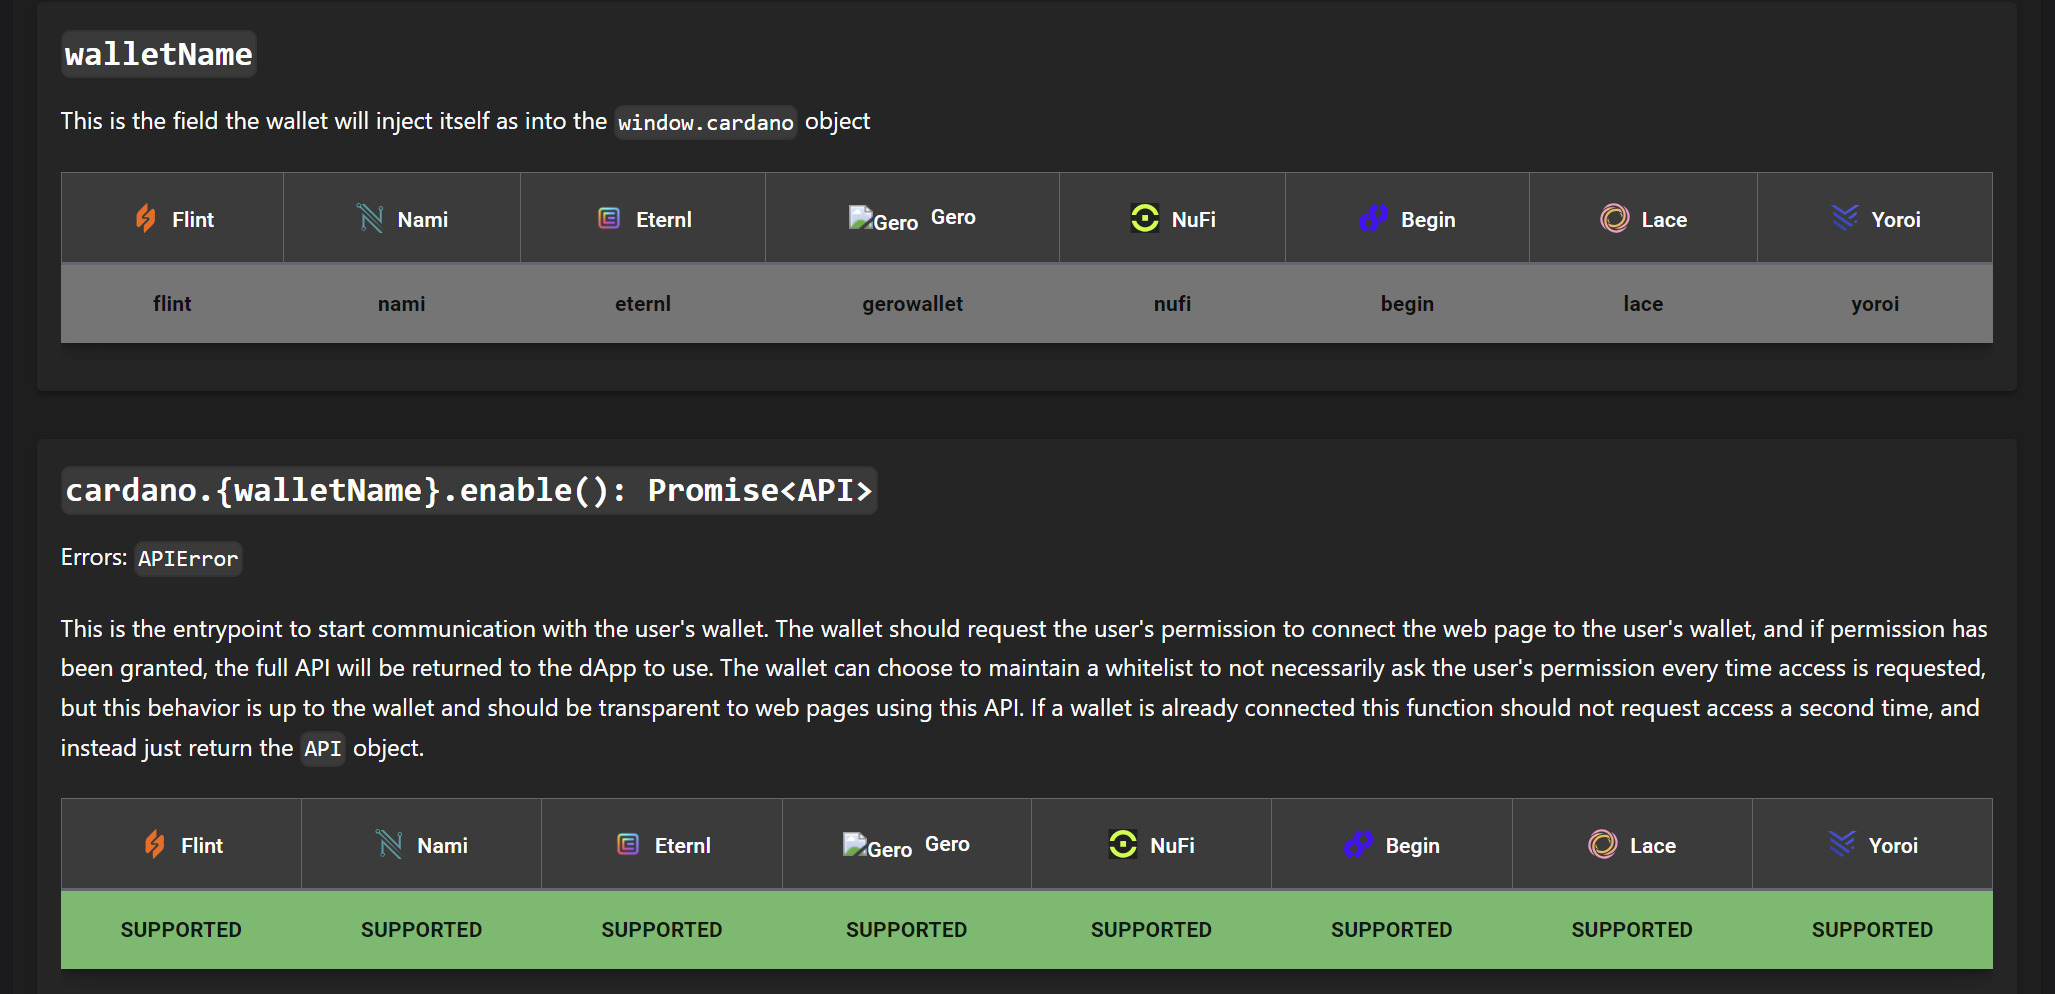
\includegraphics[scale=0.3]{cip30}

The steps to interact with a wallet following cip30 are:

\begin{itemize}
    \item \textbf{cardano.{walletName}.enable()}: we get an API object as Promise, this will create a popup message to allow the wallet to connect to the current website
    \item \textbf{api.getBalance()}: using the API object we got before, we get the total amount of Lovelace in the wallet (1 ADA = 1000,000 Lovelace)
    \item \textbf{api.signTx}: Signing a tx that was built with Lucid or any other library we sign and interact with the blockchain 
\end{itemize}

\begin{remark}
    EXERCISE 1: Create a webpage with 2 buttons, 1 to enable the wallet connection and, a second button to view the amount of ADA in the wallet.
\end{remark}




\section{Interacting with Cardano Node and Wallet APIs}

CIP30 is not enough, what if we want to get the information regarding a specific NFT in our wallet?
How to get the list of tokens inside the wallet and get information regarding their circulation supply?

We need an indexer. We could set one on our own or use a service, in this book we'll use \textbf{Maestro} as a service provider so the first thing to do is:

\subsection{Create a Maestro account}

Head over \href{https://dashboard.gomaestro.org/login}{Maestro login} page and create an account, here we'll be able to get the API keys to interact with Cardano.

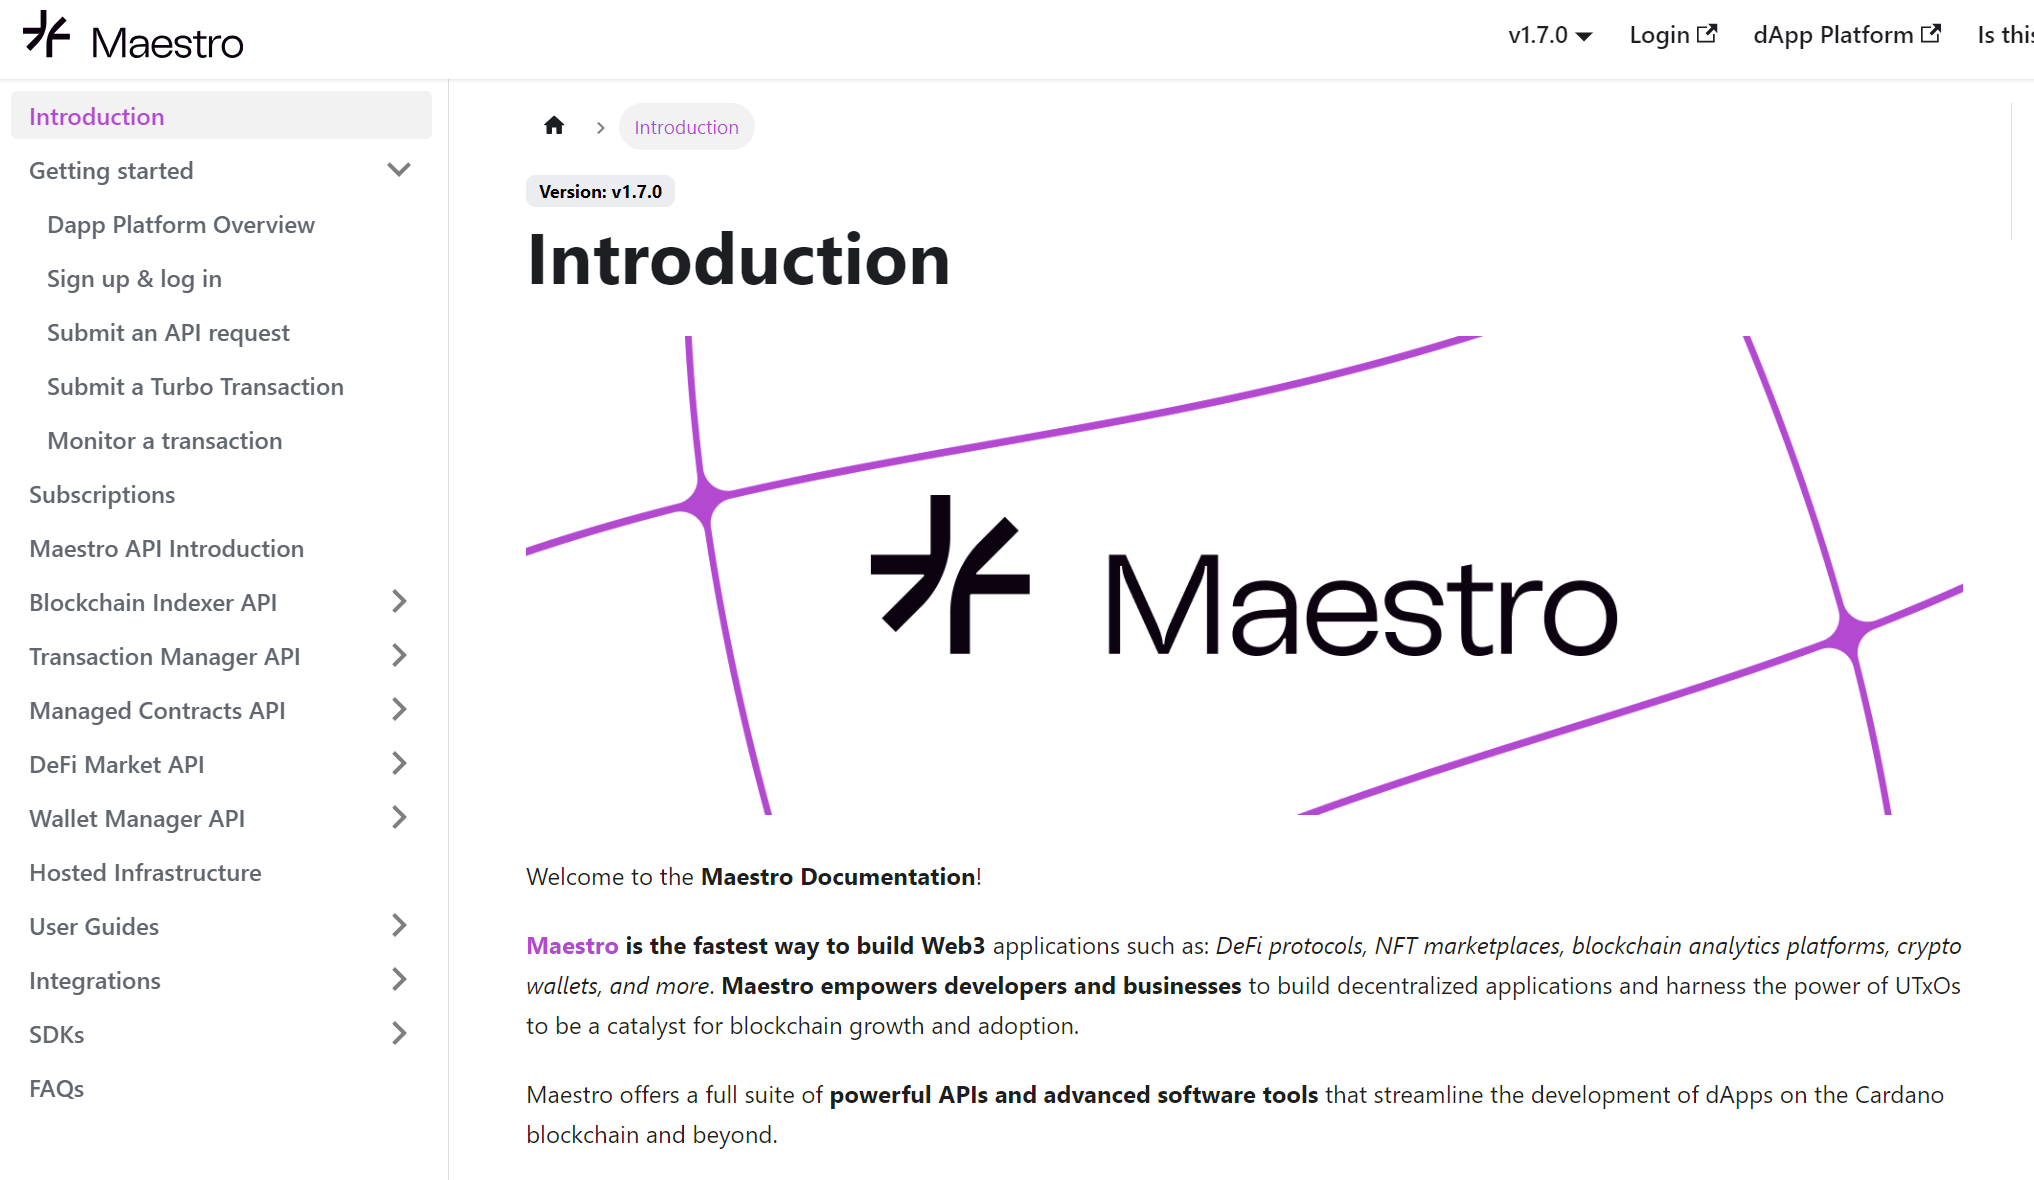
\includegraphics[scale=0.3]{maestro.png}

Maestro is going to be our key to getting all the possible APIs in order to interact with Cardano, here are the possible things we can do with these APIs:

\begin{itemize}
    \item Get the history of an address with this \href{ttps://docs.gomaestro.org/Indexer-API/Addresses/txs-by-address}{API}
    \item Get all the assets of a specific policy 
    \item Get the address holding a specific ada handle
    \item Get the history of holders for a specific NFT 
    \item and much more 
\end{itemize}

Now that we have a way to interact with a wallet and APIs to query the Cardano blockchain we are ready to put our hands on the real coding part.

\subsection{Indexer alternatives}

If you would like to explore additional API providers you should consider the following:

\begin{itemize}
    \item Blockfrost: The very first API provider for Cardano \href{https://blockfrost.io/dashboard}{link}
    \item Kupo: A tool that requires a node in order to host your own11 indexer \href{https://github.com/CardanoSolutions/kupo}{Github}
    \item Db-sync: Additional indexer that requires a Cardano Node, this is the very first one that was created \href{https://github.com/IntersectMBO/cardano-db-sync}{Github}
\end{itemize}

Now Let's code smart contracts.

\begin{remark}
    EXERCISE 2: Head over to http://cnftlab.party/ and connect your testnet wallet, mint a collection of NFTs and then use Maestro to get the information of each NFT of your collection.
\end{remark}


\section{Setting Up a Cardano Node on Contabo Cloud VPS}

\subsection{Step 1: Provisioning a Contabo Cloud VPS}
\begin{enumerate}
    \item Sign up for a Contabo Cloud VPS plan, such as the "Cloud VPS L".
    \item Once you have access to your VPS, log in via SSH.
\end{enumerate}

\subsection{Step 2: Downloading and Extracting Cardano Node Software}
\begin{enumerate}
    \item Navigate to the official Cardano GitHub release page: \href{https://github.com/input-output-hk/cardano-node/releases/tag/8.1.2}{Cardano Node Releases}.
    \item Download the Cardano Node software for macOS by running the following command:
    \begin{verbatim}
    wget https://github.com/input-output-hk/cardano-node/releases/download/8.1.2/cardano-node-8.1.2-macos.tar.gz
    \end{verbatim}
    \item After the download completes, create a directory named "node" and extract the downloaded files into it:
    \begin{verbatim}
    mkdir node
    tar xvzf cardano-node-8.1.2-macos.tar.gz -C node
    \end{verbatim}
\end{enumerate}

\subsection{Step 3: Setting Up Node Configuration}
\begin{enumerate}
    \item Create the necessary directories:
    \begin{verbatim}
    cd node
    mkdir mainnet
    cd ..
    mkdir sockets
    \end{verbatim}
    \item Create a systemd service file for the Cardano Node:
    \begin{verbatim}
    sudo nano /etc/systemd/system/cardano-node.service
    \end{verbatim}
    
    Paste the following content in the file:

    \begin{verbatim}
sudo nano /etc/systemd/system/cardano-node.service
Now we should copy and paste the following lines:
[Unit]
Description=Cardano Pool
After=multi-user.target
[Service]
Type=simple
ExecStart=/home/ubuntu/nodev30/cardano-node run --config
/home/ubuntu/nodev30/config/mainnet-config.json --topology
/home/ubuntu/nodev30/config/mainnet-topology.json --database-path
/home/ubuntu/nodev30/mainnet/db/ --socket-path  /home/ubuntu/nodev30/sockets/node.socket --
host-addr 0.0.0.0 --port 3001

KillSignal = SIGINT
RestartKillSignal = SIGINT
StandardOutput=syslog
StandardError=syslog
SyslogIdentifier=cardano
LimitNOFILE=32768

Restart=on-failure
RestartSec=15s
WorkingDirectory=~
User=USERNAMEVPS

[Install]
WantedBy=multi-user.target
    \end{verbatim}

    Save the file and exit the editor.
\end{enumerate}

\subsection{Step 4: Installing Required Dependencies and Syncing the Blockchain}
\begin{enumerate}
    \item Update package list and install necessary tools:
    \begin{verbatim}
    sudo apt update && sudo apt install liblz4-tool jq curl
    \end{verbatim}
    \item Fetch the latest blockchain snapshot and sync the blockchain:
    \begin{verbatim}
    curl -o - https://downloads.csnapshots.io/snapshots/mainnet/$(curl -s https://downloads.csnapshots.io/snapshots/mainnet/mainnet-db-snapshot.json| jq -r .[].file_name ) | lz4 -c -d - | tar -x -C /root/node/mainnet/
    \end{verbatim}
    This process may take around 30 minutes.
\end{enumerate}

\subsection{Step 5: Starting the Cardano Node}
\begin{enumerate}
    \item Enable and start the Cardano Node service:
    \begin{verbatim}
    sudo systemctl enable cardano-node.service
    sudo systemctl start cardano-node.service
    \end{verbatim}
    \item Monitor the node's status:
    \begin{verbatim}
    journalctl -u cardano-node.service -f -o cat
    \end{verbatim}
\end{enumerate}

\subsection{Step 6: Setting Up Cardano Submit API}
\begin{enumerate}
    \item Navigate to the node directory:
    \begin{verbatim}
    cd node
    \end{verbatim}
    \item Create a configuration file for the transaction submission API:
    \begin{verbatim}
    nano tx-submit-mainnet-config.yaml
    \end{verbatim}
    Paste the content from \href{https://github.com/input-output-hk/cardano-node/blob/master/cardano-submit-api/config/tx-submit-mainnet-config.yaml}{Cardano Node GitHub} into this file. Save and exit the editor.
    \item Run the Cardano Submit API with the provided configuration:
    \begin{verbatim}
    ./cardano-submit-api --tx-submit-mainnet-config.yaml --socket-path /root/node/sockets/socket node.socket --port 8090 --mainnet --host-addr 0.0.0.0
    \end{verbatim}
\end{enumerate}

\subsection{Step 7: Accessing Transaction Submission Endpoint}
With the Cardano Submit API running, you can now send transactions using your node by accessing the following URL:
\begin{verbatim}
http://VPSIPADDRESS:8090/api/submit/tx
\end{verbatim}
Replace \texttt{VPSIPADDRESS} with the IP address of your VPS.

By following these steps, you'll have successfully set up a Cardano node on your Contabo Cloud VPS and be ready to interact with the Cardano blockchain.



\newpage
\part{EXERCISE solutions}
\chapter{Solutions}
\section{Solutions}

\subsection{Exercise 1}
\textit{You can find the solution file for easy copy and paste:} \href{https://github.com/elRaulito/eUTxO-Fundamentals-Building-Cardano-Smart-Contracts/blob/main/eBook/sections/solutions/index.html}{Solution 1 File (formatted code)}


% Define HTML language style for listings
\lstdefinelanguage{HTML}{
    sensitive=true,
    keywords={},
    otherkeywords={<, >, /, =},
    morecomment=[s]{<!--}{-->},
    morestring=[b]",
    morestring=[b]',
}

% Set listing style
\lstset{
    basicstyle=\ttfamily\small,
    commentstyle=\color{gray},
    stringstyle=\color{blue},
    keywordstyle=\color{black},
    showstringspaces=false,
    tabsize=4,
    language=HTML,
    breaklines=true,
    frame=single,
    captionpos=b
}


\lstinputlisting[]{sections/solutions/index.html}

\subsection{Exercise 2}
\textit{You can find the solution file for easy copy and paste:} \href{https://github.com/elRaulito/eUTxO-Fundamentals-Building-Cardano-Smart-Contracts/blob/main/eBook/sections/solutions/get_addresses.py}{Solution 2 File (formatted code)}

% Define Python language style for listings
\lstdefinelanguage{Python}{
  keywords={import, def, while, True, if, else, break, print, with, as, not, None},
  keywordstyle=\color{blue}\bfseries,
  ndkeywords={class, return, try, except, finally, raise},
  ndkeywordstyle=\color{orange}\bfseries,
  identifierstyle=\color{black},
  sensitive=false,
  comment=[l]{\#},
  morecomment=[s]{/*}{*/},
  commentstyle=\color{gray}\ttfamily,
  stringstyle=\color{red}\ttfamily,
  morestring=[b]',
  morestring=[b]"
}

% Set listing style
\lstset{
  basicstyle=\ttfamily\small,
  commentstyle=\color{gray},
  stringstyle=\color{green},
  keywordstyle=\color{blue},
  showstringspaces=false,
  tabsize=4,
  language=Python,
  breaklines=true,
  frame=single,
  captionpos=b
}


\lstinputlisting[]{sections/solutions/get_addresses.py}


\subsection{Exercise 3}
\textit{You can find the solution file for easy copy and paste:} \href{https://github.com/elRaulito/eUTxO-Fundamentals-Building-Cardano-Smart-Contracts/blob/main/eBook/sections/solutions/nft.ak}{Solution 3 File (formatted code)}
% Define Aiken language style for listings
\lstdefinelanguage{Aiken} {
    keywords={
        use, pub, type, validator, fn, let, if, else, when, trace, expect, and, or, fail, True, False,
        Mint, Burn, Action, Option, List, Dict, Pair, ByteArray, Int, Pairs, Input, Output, Transaction, Script, NoDatum
    },
    keywordstyle=\color{blue}\bfseries,
    ndkeywords={
        from_asset, from_asset_list, mock_policy_id, mock_pub_key_hash, mock_utxo_ref, assets, dict, list, to_string, to_bytearray
    },
    ndkeywordstyle=\color{orange}\bfseries,
    identifierstyle=\color{black},
    sensitive=false,
    comment=[l]{\#},
    morecomment=[s]{/*}{*/},
    commentstyle=\color{gray}\ttfamily,
    stringstyle=\color{red}\ttfamily,
    morestring=[b]',
    morestring=[b]"
}

% Set listing style for Aiken code
\lstset{
    basicstyle=\ttfamily\small,
    commentstyle=\color{gray},
    stringstyle=\color{red},
    keywordstyle=\color{blue},
    showstringspaces=false,
    tabsize=4,
    language=Aiken,
    breaklines=true,
    frame=single,
    captionpos=b
}



\lstinputlisting[]{sections/solutions/nft.ak}

\subsection{Exercise 4}
\textit{You can find the solution file for easy copy and paste:} \href{https://github.com/elRaulito/eUTxO-Fundamentals-Building-Cardano-Smart-Contracts/blob/main/eBook/sections/solutions/cip69.ak}{Solution 4 File (formatted code)}
% Define Aiken language style for listings
\lstdefinelanguage{Aiken} {
    keywords={
        use, pub, type, validator, fn, let, if, else, when, trace, expect, and, or, fail, True, False,
        Mint, Burn, Action, Option, List, Dict, Pair, ByteArray, Int, Pairs, Input, Output, Transaction, Script, NoDatum
    },
    keywordstyle=\color{blue}\bfseries,
    ndkeywords={
        from_asset, from_asset_list, mock_policy_id, mock_pub_key_hash, mock_utxo_ref, assets, dict, list, to_string, to_bytearray
    },
    ndkeywordstyle=\color{orange}\bfseries,
    identifierstyle=\color{black},
    sensitive=false,
    comment=[l]{\#},
    morecomment=[s]{/*}{*/},
    commentstyle=\color{gray}\ttfamily,
    stringstyle=\color{red}\ttfamily,
    morestring=[b]',
    morestring=[b]"
}

% Set listing style for Aiken code
\lstset{
    basicstyle=\ttfamily\small,
    commentstyle=\color{gray},
    stringstyle=\color{red},
    keywordstyle=\color{blue},
    showstringspaces=false,
    tabsize=4,
    language=Aiken,
    breaklines=true,
    frame=single,
    captionpos=b
}



\lstinputlisting[]{sections/solutions/cip69.ak}

\subsection{Exercise 5}
\textit{You can find the solution file for easy copy and paste:} \href{https://github.com/elRaulito/eUTxO-Fundamentals-Building-Cardano-Smart-Contracts/blob/main/eBook/sections/solutions/fraction.ak}{Solution 5 File (formatted code)}
% Define Aiken language style for listings
\lstdefinelanguage{Aiken} {
    keywords={
        use, pub, type, validator, fn, let, if, else, when, trace, expect, and, or, fail, True, False,
        Mint, Burn, Action, Option, List, Dict, Pair, ByteArray, Int, Pairs, Input, Output, Transaction, Script, NoDatum
    },
    keywordstyle=\color{blue}\bfseries,
    ndkeywords={
        from_asset, from_asset_list, mock_policy_id, mock_pub_key_hash, mock_utxo_ref, assets, dict, list, to_string, to_bytearray
    },
    ndkeywordstyle=\color{orange}\bfseries,
    identifierstyle=\color{black},
    sensitive=false,
    comment=[l]{\#},
    morecomment=[s]{/*}{*/},
    commentstyle=\color{gray}\ttfamily,
    stringstyle=\color{red}\ttfamily,
    morestring=[b]',
    morestring=[b]"
}

% Set listing style for Aiken code
\lstset{
    basicstyle=\ttfamily\small,
    commentstyle=\color{gray},
    stringstyle=\color{red},
    keywordstyle=\color{blue},
    showstringspaces=false,
    tabsize=4,
    language=Aiken,
    breaklines=true,
    frame=single,
    captionpos=b
}



\lstinputlisting[]{sections/solutions/fraction.ak}




\newglossaryentry{Determinism}{
    name=Determinism,
    description={Transaction and blockchain behavior are predictable, given a sort of input and outputs, once the fee is decided the transaction hash will always be the same}
}
\newglossaryentry{Composability}{
    name=Composability,
    description={Also referred to as transaction in transaction, it's the ability to interact with multiple parties in the same transaction, this is not possible in the account model, however, this also raises the concurrency issue when two parties or transactions want to spend the same utxo}
}
\newglossaryentry{Liquid Staking}{
    name=Liquid Staking,
    description={Cardano staking is referred to as Liquid, no locking mechanism is needed to get the staking rewards. This becomes useful because users can move their ADA around inside smart contracts while keeping the delegation rewards }
}
\newglossaryentry{orderbook}{
    name=orderbook,
    description={In this configuration each order placed by users is a single entry with a price and amount of token willing to sell (ADA or native tokens), swaps happen matching the orders }
}
\newglossaryentry{AMM}{
    name=AMM,
    description={Automatic market maker dexes involve a liquidity pool, the pool has two pair tokens, usually ADA and the Cardano native token, users can sell or buy tokens from this pool and the price is adjusted according to the market need }
}

\newglossaryentry{CIP}{
    name=CIP,
    description={Cardano Improvement Proposals that if approved can change the current ledger or chain parameters, usually are also standards to develop in a similar way between projects  }
}

\newglossaryentry{inputs}{
    name=inputs,
    description={Inputs in a UTXO model transaction specify which unspent outputs are being consumed, so which funds coming from previous transactions are being spent. }
}

\newglossaryentry{epoch}{
    name=epoch,
    description={An epoch in Cardano is a fixed period during which a set of blocks is produced. The duration of an epoch is predefined and consistent. As of the current Cardano implementation, an epoch lasts for 5 days. At the end of each epoch, rewards are calculated and distributed, and a new epoch begins. Epochs help structure the blockchain into manageable time periods, enabling efficient consensus and reward mechanisms.
    }
}

\newglossaryentry{block}{
    name=block,
    description={A block in Cardano is a record of transactions and other information produced by a slot leader during a slot. Blocks are added to the blockchain sequentially. Each block contains a header with metadata, such as the previous block hash, and a body that includes the transaction data and other relevant information. Blocks are produced by slot leaders, which are chosen through the Ouroboros consensus protocol, Cardano's proof-of-stake mechanism. Blocks are essential for maintaining the integrity and continuity of the blockchain, as they confirm and validate transactions.
    }
}


\newglossaryentry{slot}{
    name=slot,
    description={A slot is a smaller time unit within an epoch. An epoch is divided into a large number of slots. Each slot represents a potential opportunity to produce a block. In the current implementation of Cardano, there are 432,000 slots in an epoch, with each slot lasting 1 second. However, not every slot will necessarily have a block produced, as block production depends on the consensus protocol and slot leader election.
    }
}
\printglossary[title={Glossary}, type=main]
\end{document}
